\section*{Laporan Hasil Percobaan Wireless} % Judul sederhana tanpa nomor
\addcontentsline{toc}{section}{Laporan Hasil Percobaan Wireless} % Menambahkan ke Daftar Isi jika ada

\section{Langkah-Langkah Percobaan}
Pada praktikum ini, dilakukan tiga skenario konfigurasi jaringan nirkabel. Setiap skenario diawali dengan mereset router ke pengaturan awal untuk menghindari konflik konfigurasi, diikuti dengan proses login ke router.

\subsection*{$\bullet$ Wireless Point-to-Point}
\addcontentsline{toc}{subsection}{Wireless Point-to-Point}
Proses konfigurasi dimulai dengan mengatur Router A.
\begin{enumerate}
    \item Router A disetel sebagai \textbf{Bridge} melalui antarmuka \textit{Wireless -> Wifi Interface}, dengan SSID \texttt{PointToPoint\_2}.
    \begin{center}
        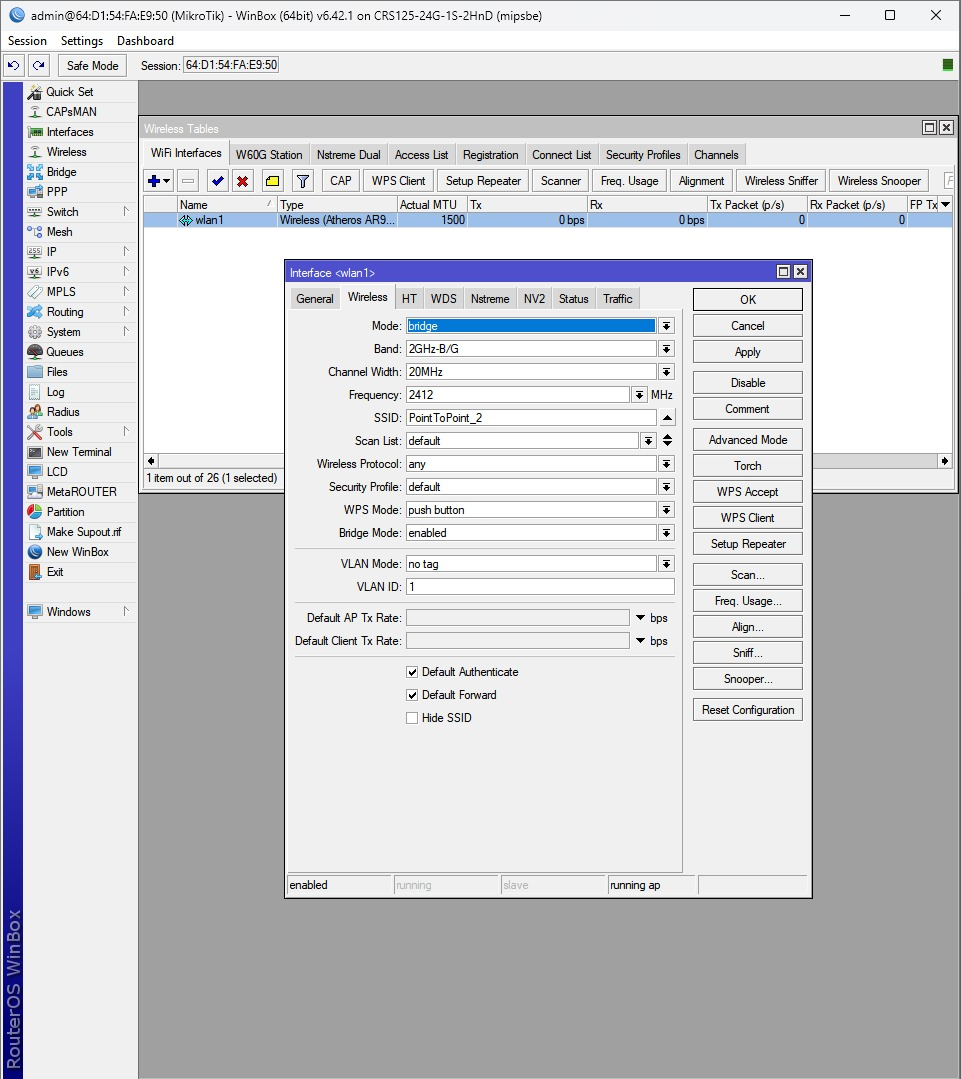
\includegraphics[width=0.5\textwidth]{img/bridge.jpg}
        \captionof{figure}{Pengaturan Router A sebagai Bridge}
    \end{center}
    \item Router B kemudian dikonfigurasi sebagai \textbf{Station}.
    \item Dari Router B, dilakukan pemindaian (\textit{scan}) jaringan nirkabel. SSID \texttt{PointToPoint\_2} dipilih dan dihubungkan (\textit{connect}).
    \item Alamat IP untuk antarmuka WLAN1 pada Router A diatur menjadi \texttt{10.10.10.1/29}.
    \item Alamat IP untuk antarmuka WLAN1 pada Router B diatur menjadi \texttt{10.10.10.2/29}.
    \item Selanjutnya, IP LAN (interface ether1) Router A disetel ke \texttt{192.168.20.1/24}.
    \item IP LAN (interface ether1) Router B disetel ke \texttt{192.168.30.1/24}.
    \item Laptop yang terhubung ke Router A diberikan IP \texttt{192.168.20.2/24}.
    \item Laptop yang terhubung ke Router B diberikan IP \texttt{192.168.30.2/24}.
    \item Konfigurasi routing ditambahkan melalui menu \textit{Routing -> Address} (atau \textit{IP -> Routes}).
    \item Alamat IP network tujuan (misalnya \texttt{192.168.30.0/24} di Router A, dan \texttt{192.168.20.0/24} di Router B) ditambahkan ke tabel routing, dengan gateway berupa IP WLAN router tetangga.
    \begin{center}
        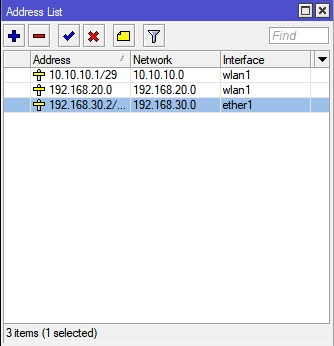
\includegraphics[width=0.5\textwidth]{img/address.jpg}
        \captionof{figure}{Penambahan alamat pada tabel routing}
    \end{center}
    \item Pengujian konektivitas dilakukan dengan \texttt{ping} antar router.
    \begin{center}
        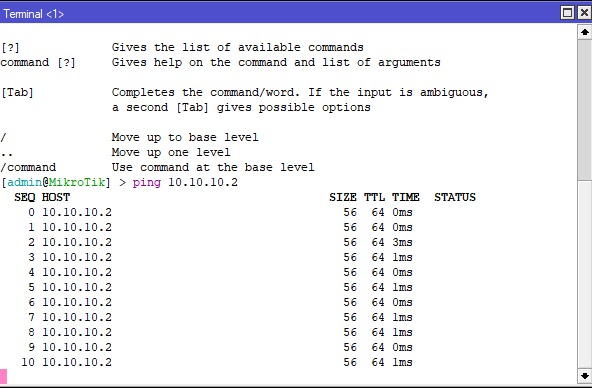
\includegraphics[width=0.4\textwidth]{img/pingrslt3.jpg}
        \captionof{figure}{Hasil uji ping antar router (P2P)}
    \end{center}
    \item Pengujian dilanjutkan dengan \texttt{ping} antar PC yang terhubung ke masing-masing router.
    \begin{center}
        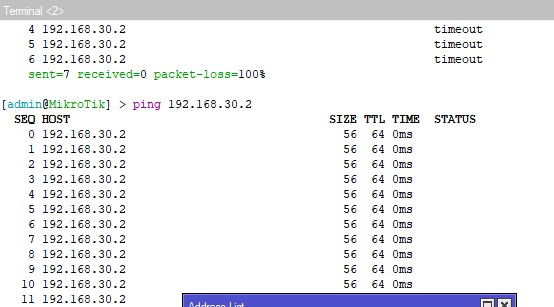
\includegraphics[width=0.7\textwidth]{img/pingrslt2.jpg} % Lebar disesuaikan agar tidak terlalu besar
        \captionof{figure}{Hasil uji ping antar PC (P2P)}
    \end{center}
\end{enumerate}

\subsection*{$\bullet$ Wireless Point-to-Multipoint}
\addcontentsline{toc}{subsection}{Wireless Point-to-Multipoint}
Skenario ini bertujuan menghubungkan beberapa perangkat ke satu titik akses.
\begin{enumerate}
    \item Setelah reset dan login, Router A dikonfigurasi sebagai \textbf{AP Bridge} melalui \textit{Wireless -> Wifi Interface}, dengan SSID \texttt{PointToPoint\_2}.
    \begin{center}
        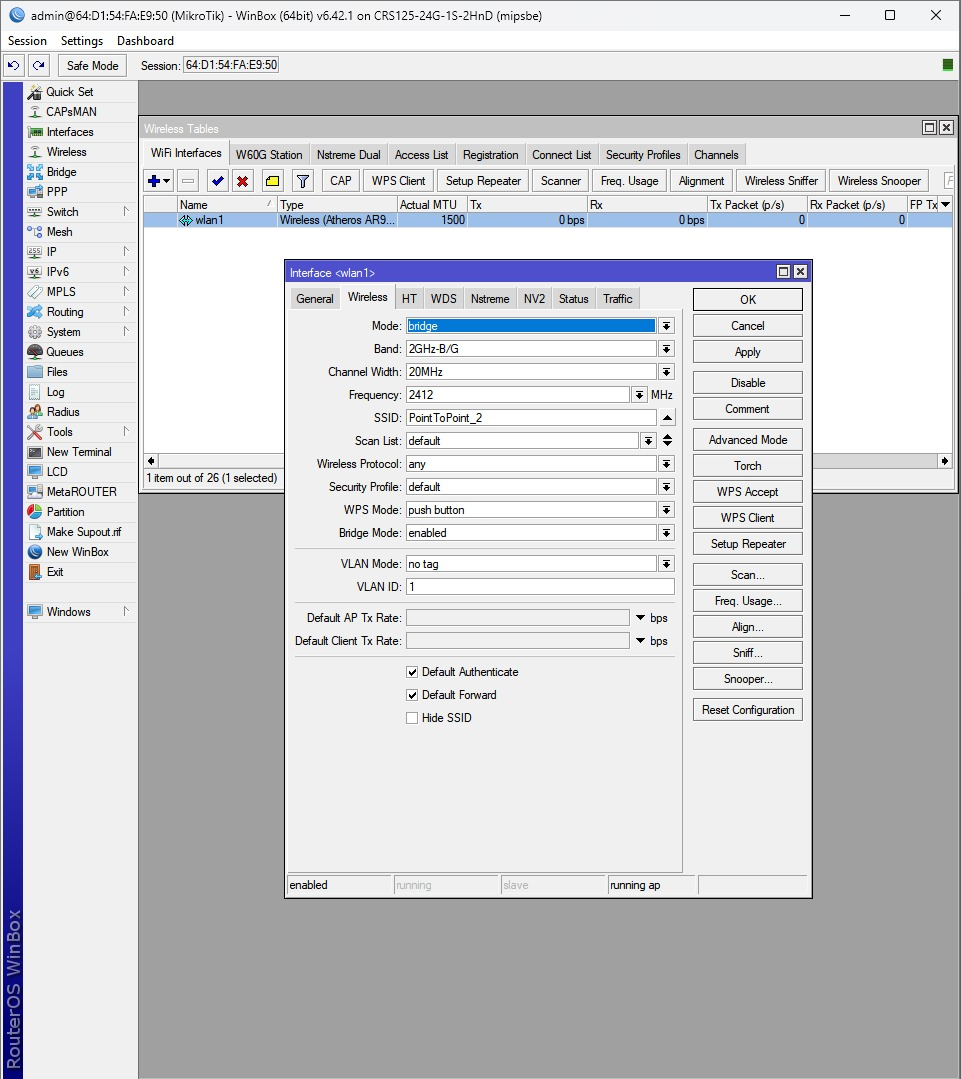
\includegraphics[width=0.5\textwidth]{img/bridge.jpg} % Gambar sama dengan P2P untuk mode AP Bridge
        \captionof{figure}{Pengaturan Router A sebagai AP Bridge}
    \end{center}
    \item Router B diatur sebagai \textbf{Station}.
    \item Dari Router B, dilakukan \textit{scan} untuk SSID \texttt{PointToPoint\_2}, lalu dihubungkan. Setelah terhubung, status router klien ini dapat terlihat sebagai terhubung ke AP (misalnya, mode berubah menjadi \textit{Station Bridge} atau sejenisnya).
    \item IP WLAN1 Router A diatur ke \texttt{10.10.10.1/29}.
    \item IP WLAN1 Router B diatur ke \texttt{10.10.10.2/29}.
    \item IP LAN (ether1) Router A disetel ke \texttt{192.168.20.1/24}.
    \item IP LAN (ether1) Router B disetel ke \texttt{192.168.30.1/24}.
    \item Laptop pada jaringan Router A diberikan IP \texttt{192.168.20.2/24}.
    \item Laptop pada jaringan Router B diberikan IP \texttt{192.168.30.2/24}.
    \item Konfigurasi routing statis ditambahkan seperti pada skenario P2P untuk menghubungkan kedua LAN.
    \begin{center}
        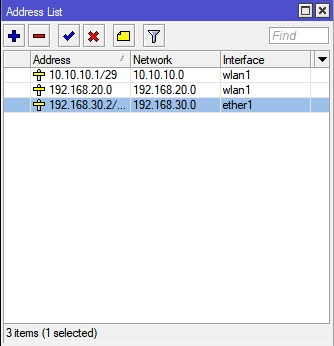
\includegraphics[width=0.5\textwidth]{img/address.jpg} % Gambar sama dengan P2P
        \captionof{figure}{Penambahan alamat routing (P2MP)}
    \end{center}
    \item Uji \texttt{ping} antar router dilakukan untuk verifikasi koneksi nirkabel.
    \begin{center}
        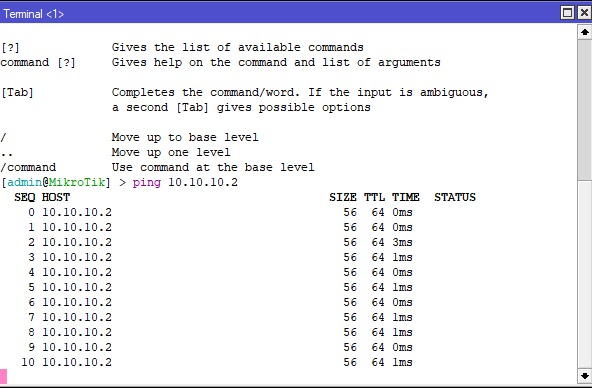
\includegraphics[width=0.4\textwidth]{img/pingrslt3.jpg} % Gambar sama dengan P2P
        \captionof{figure}{Hasil uji ping antar router (P2MP)}
    \end{center}
    \item Uji \texttt{ping} antar PC dilakukan untuk verifikasi konektivitas end-to-end.
    \begin{center}
        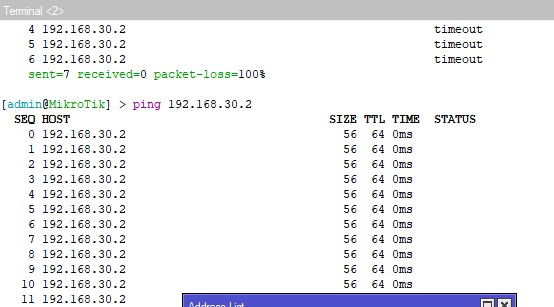
\includegraphics[width=0.7\textwidth]{img/pingrslt2.jpg} % Gambar sama dengan P2P, lebar disesuaikan
        \captionof{figure}{Hasil uji ping antar PC (P2MP)}
    \end{center}
\end{enumerate}

\subsection*{$\bullet$ Wireless Bridge}
\addcontentsline{toc}{subsection}{Wireless Bridge}
Skenario ini bertujuan menggabungkan dua jaringan LAN menjadi satu segmen.
\begin{enumerate}
    \item Router A diatur sebagai \textbf{Bridge} melalui \textit{Wireless -> Wifi Interface}, dengan SSID \texttt{PointToPoint\_2}.
    \begin{center}
        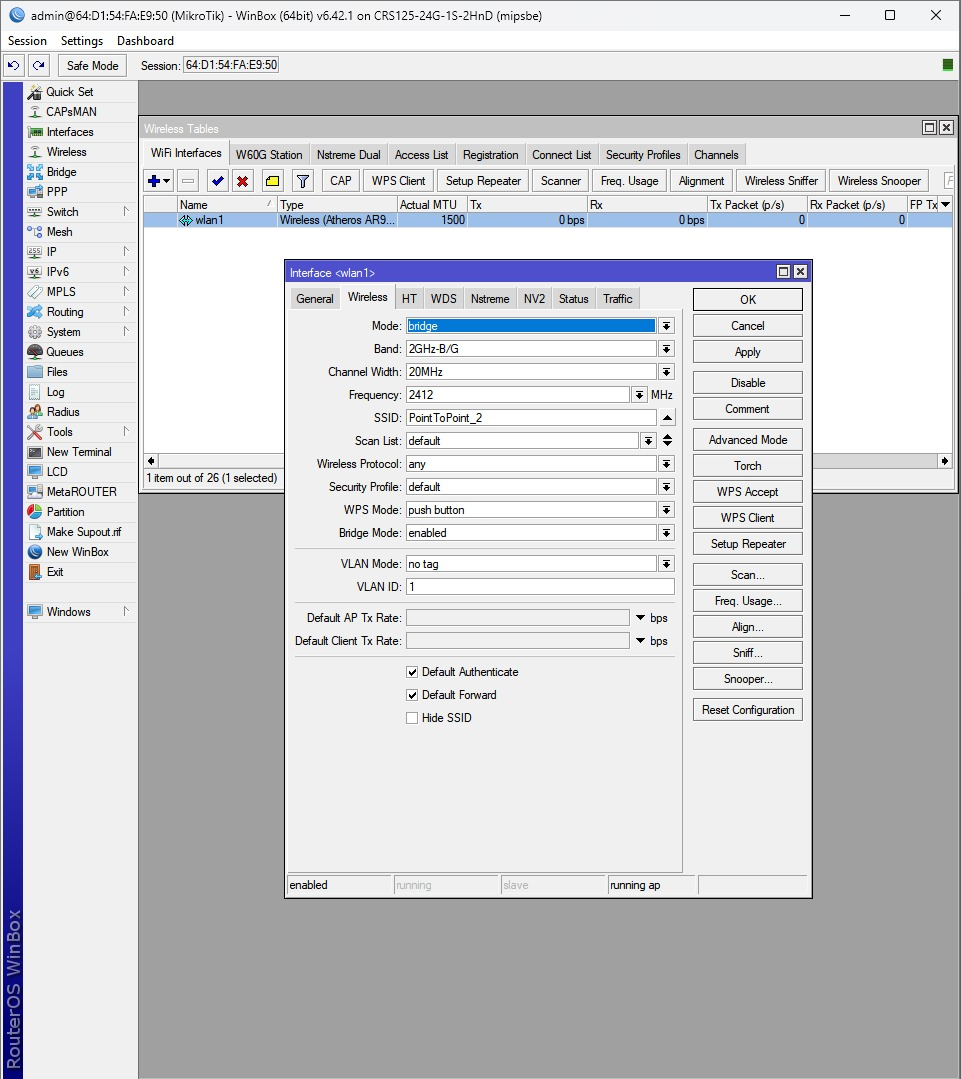
\includegraphics[width=0.5\textwidth]{img/bridge.jpg} % Gambar sama
        \captionof{figure}{Pengaturan Router A sebagai Bridge (Wireless Bridge)}
    \end{center}
    \item Router B dikonfigurasi sebagai \textbf{Station Pseudobridge}.
    \item Dari Router B, dilakukan \textit{scan} untuk SSID \texttt{PointToPoint\_2} dan dihubungkan.
    \item IP WLAN1 Router A disetel ke \texttt{10.10.10.1/29}.
    \item IP WLAN1 Router B disetel ke \texttt{10.10.10.2/29}.
    \item IP LAN (ether1) Router A diatur ke \texttt{192.168.10.2/24}. % Subnet berbeda dari P2P/P2MP
    \item IP LAN (ether1) Router B diatur ke \texttt{192.168.10.3/24}. % Subnet sama dengan Router A LAN
    \item Laptop pada jaringan Router A diberikan IP \texttt{192.168.10.5/24}.
    \item Laptop pada jaringan Router B diberikan IP \texttt{192.168.10.7/24}.
    \item Interface bridge virtual (\texttt{bridge1}) dibuat pada kedua router. Antarmuka \texttt{wlan1} dan \texttt{ether1} (atau \texttt{ether2} jika itu yang digunakan untuk LAN) ditambahkan sebagai port ke dalam \texttt{bridge1} ini. (*Catatan: Jika bridging L2 berhasil, routing statis untuk subnet LAN yang sama seharusnya tidak diperlukan lagi.*)
    \item Alamat IP network (\texttt{192.168.10.0/24}) ditambahkan ke tabel routing.
    \begin{center}
        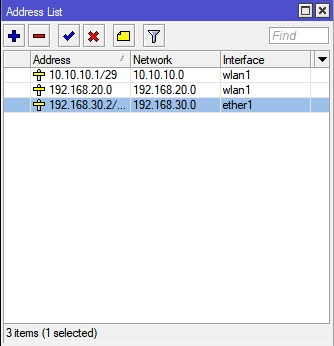
\includegraphics[width=0.5\textwidth]{img/address.jpg} % Gambar sama
        \captionof{figure}{Penambahan alamat routing (Wireless Bridge)}
    \end{center}
    \item Uji \texttt{ping} antar router (menggunakan IP WLAN) diverifikasi.
    \begin{center}
        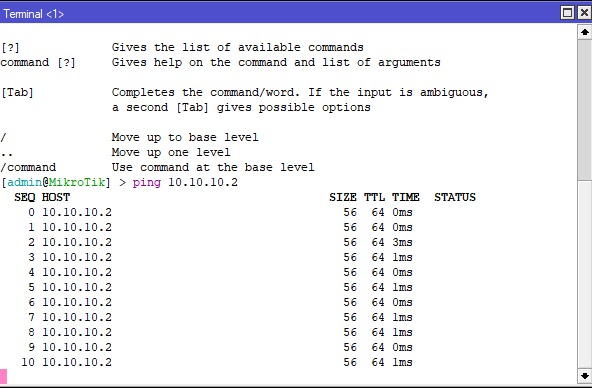
\includegraphics[width=0.4\textwidth]{img/pingrslt3.jpg} % Gambar sama
        \captionof{figure}{Hasil uji ping antar router (Wireless Bridge)}
    \end{center}
    \item Uji \texttt{ping} antar PC (misalnya, dari \texttt{192.168.10.5} ke \texttt{192.168.10.7}) dilakukan.
    \begin{center}
        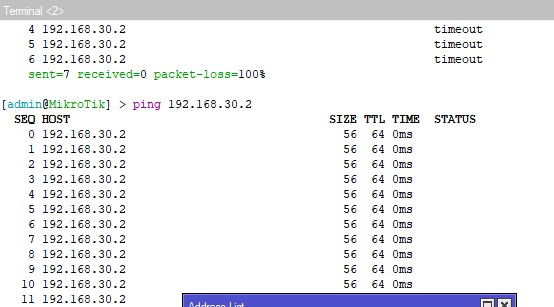
\includegraphics[width=0.7\textwidth]{img/pingrslt2.jpg} % Gambar sama, lebar disesuaikan
        \captionof{figure}{Hasil uji ping antar PC (Wireless Bridge)}
    \end{center}
\end{enumerate}

\section{Analisis Hasil Percobaan}
Pada ketiga percobaan yang telah dilaksanakan, dilakukan analisis sebagai berikut:

\subsection*{$\bullet$ Point-to-Point}
\addcontentsline{toc}{subsection}{Analisis Point-to-Point}
Dalam konfigurasi ini, satu router berfungsi sebagai \textit{bridge} dan yang lainnya sebagai \textit{station}. Hasil uji \texttt{ping} antar router yang berhasil menunjukkan bahwa tautan nirkabel langsung dan routing statis antar kedua LAN telah sukses dikonfigurasi.

\subsection*{$\bullet$ Point-to-Multipoint}
\addcontentsline{toc}{subsection}{Analisis Point-to-Multipoint}
Satu router diatur sebagai \textit{AP bridge} dan satu lainnya sebagai \textit{station} (yang kemudian terhubung sebagai \textit{AP station} atau klien AP). Meskipun mode \textit{AP bridge} dirancang untuk melayani beberapa klien, pengujian hanya melibatkan satu klien karena keterbatasan perangkat. Namun, uji \texttt{ping} antar router yang berhasil mengindikasikan bahwa koneksi dasar dan routing untuk skenario dengan satu stasiun ini telah berfungsi dengan baik.

\subsection*{$\bullet$ Wireless Bridge}
\addcontentsline{toc}{subsection}{Analisis Wireless Bridge}
Dengan satu router sebagai \textit{Bridge} dan lainnya sebagai \textit{Station Pseudobridge}, diharapkan terbentuk jembatan Layer 2 yang transparan. Uji \texttt{ping} antar alamat IP WLAN router berhasil dilakukan. Meskipun pengujian mendalam terhadap fungsionalitas bridge L2 (seperti verifikasi tabel MAC) tidak dilakukan, keberhasilan ping antar router menandakan tautan nirkabel telah terbentuk. Keberhasilan ping antar PC pada subnet yang sama juga mengindikasikan fungsi bridge berjalan.

\section{=Tugas Modul (Simulasi Jaringan Antar Gedung)}
\label{sec:tugmod_simulasi}

Pada bagian tugas modul ini, dilakukan simulasi perancangan jaringan nirkabel yang menghubungkan tiga gedung utama: Gedung Pusat, Gedung Lab, dan Gedung Asrama. Gedung Asrama sendiri dibagi lagi menjadi dua blok, yaitu Blok A dan Blok B, yang mana koneksi internal antar blok ini menjadi salah
satu fokus dalam simulasi.

\subsection{Langkah-Langkah Umum Simulasi}
Simulasi ini dirancang menggunakan perangkat lunak Cisco Packet Tracer. Langkah-langkah kunci dalam membangun topologi ini meliputi:
\begin{enumerate}
    \item \textbf{Penempatan Perangkat Utama:} Setiap gedung (Pusat, Lab, dan Asrama Blok A) dilengkapi dengan sebuah router nirkabel (misalnya, Linksys WRT300N) yang berfungsi sebagai gateway lokal dan titik akses nirkabel (AP) untuk perangkat di dalamnya. Gedung Asrama Blok B juga dilengkapi dengan AP lokal.
    \item \textbf{Konfigurasi Jaringan Lokal (LAN) Setiap Gedung:}
        \begin{itemize}
            \item Router di setiap gedung dikonfigurasi dengan subnet IP yang unik untuk LAN masing-masing (misalnya, Gedung Pusat: \texttt{192.168.1.0/24}, Gedung Lab: \texttt{192.168.2.0/24}, Gedung Asrama (A\&B): \texttt{192.168.3.0/24}).
            \item DHCP server diaktifkan pada setiap router utama gedung untuk distribusi IP otomatis ke klien.
            \item SSID dan keamanan nirkabel (WPA2-PSK) dikonfigurasi pada setiap AP.
        \end{itemize}
    \item \textbf{Interkoneksi Antar Gedung:}
        \begin{itemize}
            \item Router Gedung Lab dan router utama Gedung Asrama (di Blok A) dihubungkan ke jaringan lokal Gedung Pusat. Port WAN dari router Lab dan Asrama A dikonfigurasi dengan IP statis yang berada dalam subnet LAN Gedung Pusat, dengan gateway mengarah ke router Gedung Pusat.
            \item Rute statis ditambahkan pada router Gedung Pusat untuk mengenali subnet LAN Gedung Lab dan Gedung Asrama.
        \end{itemize}
    \item \textbf{Koneksi Internal Gedung Asrama (Blok A ke Blok B):}
        Sesuai pembahasan kita, koneksi antara Blok A dan Blok B di Gedung Asrama semula direncanakan menggunakan wireless bridge (menggunakan dua perangkat AP-PT). Namun, karena kendala teknis dalam simulasi Packet Tracer dimana link nirkabel antar AP-PT tersebut tidak terbentuk meskipun konfigurasi telah diverifikasi berkali-kali, maka sebagai alternatif fungsional, koneksi antara switch di Blok A dan switch di Blok B dilakukan menggunakan kabel Ethernet. Hal ini memastikan Blok A dan B tetap berada dalam satu segmen LAN yang sama (\texttt{192.168.3.0/24}) dan dilayani oleh router utama di Blok A.
    \item \textbf{Penempatan dan Konfigurasi End Devices:} Laptop atau PC ditambahkan di setiap gedung/blok dan dikonfigurasi untuk terhubung ke jaringan nirkabel lokal masing-masing serta mendapatkan konfigurasi IP melalui DHCP.
    \item \textbf{Pengujian Konektivitas:} Dilakukan uji ping antar perangkat dalam satu LAN, antar LAN di gedung berbeda, dan khususnya antar Blok A dan B di Gedung Asrama.
\end{enumerate}

\subsection{Visualisasi Konfigurasi dan Topologi}

Berikut adalah beberapa tangkapan layar yang merepresentasikan konfigurasi kunci dalam simulasi:

\begin{figure}[h!]
    \centering
    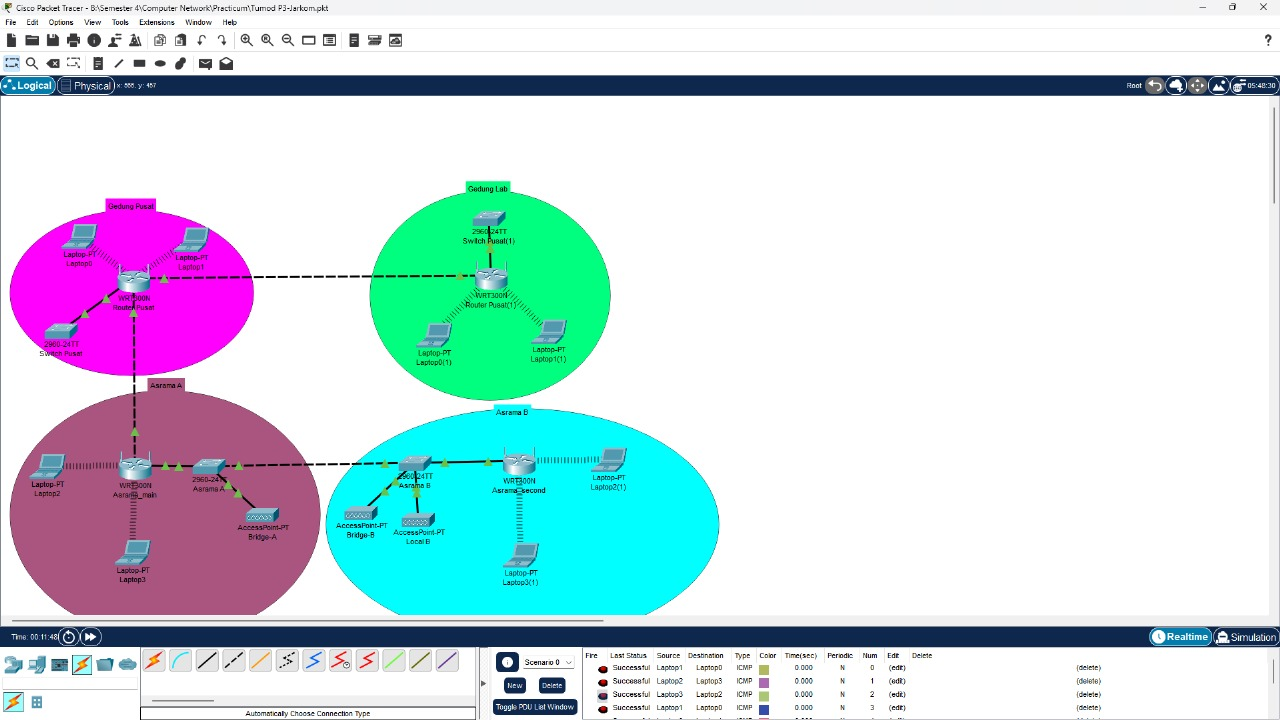
\includegraphics[width=0.8\textwidth]{img/Topologi.jpeg} 
    \caption{Topologi jaringan keseluruhan yang menghubungkan Gedung Pusat, Lab, dan Asrama (Blok A \& B). Terlihat bagaimana setiap gedung terhubung ke jaringan pusat, dan koneksi internal Asrama.}
    \label{fig:topologi_simulasi_keseluruhan}
\end{figure}
\clearpage 

\begin{figure}[h!]
    \centering
    \begin{minipage}{0.48\textwidth}
        \centering
        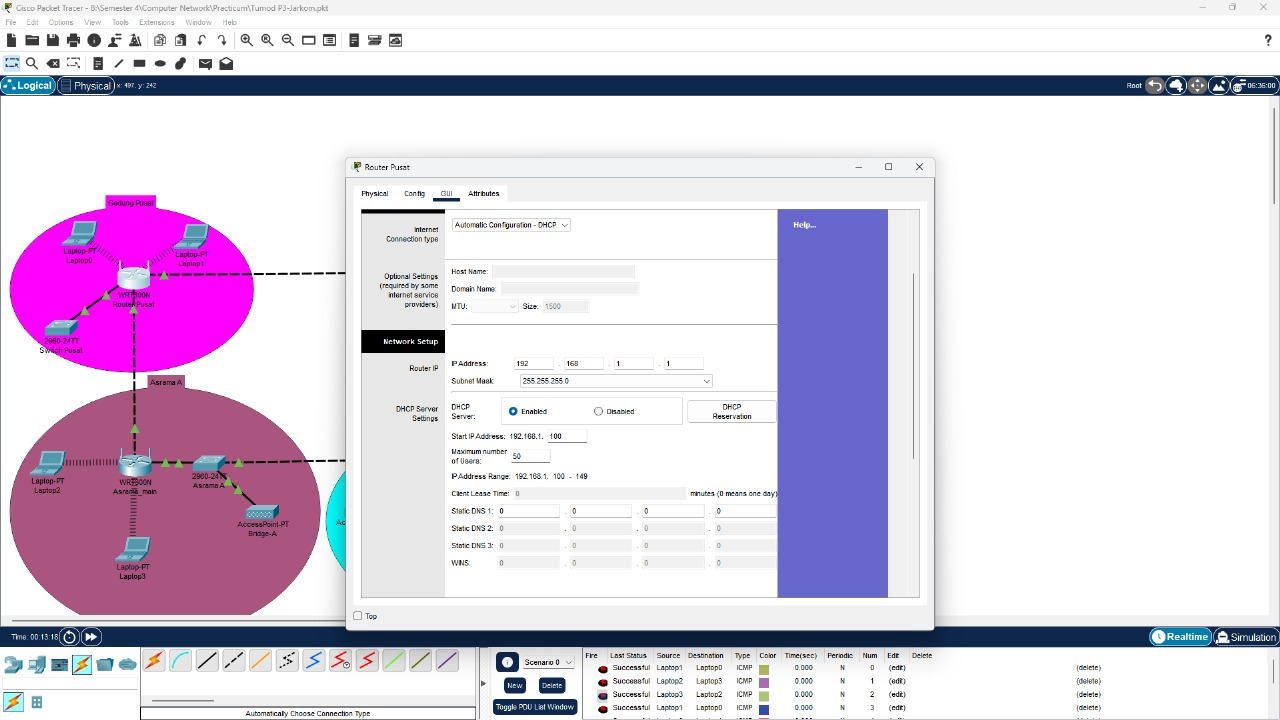
\includegraphics[width=0.6\textwidth]{img/Pusat_R.jpeg}
        \caption*{Konfigurasi Router Pusat}
        \label{fig:cfg_router_pusat}
    \end{minipage}\hfill
    \begin{minipage}{0.48\textwidth}
        \centering
        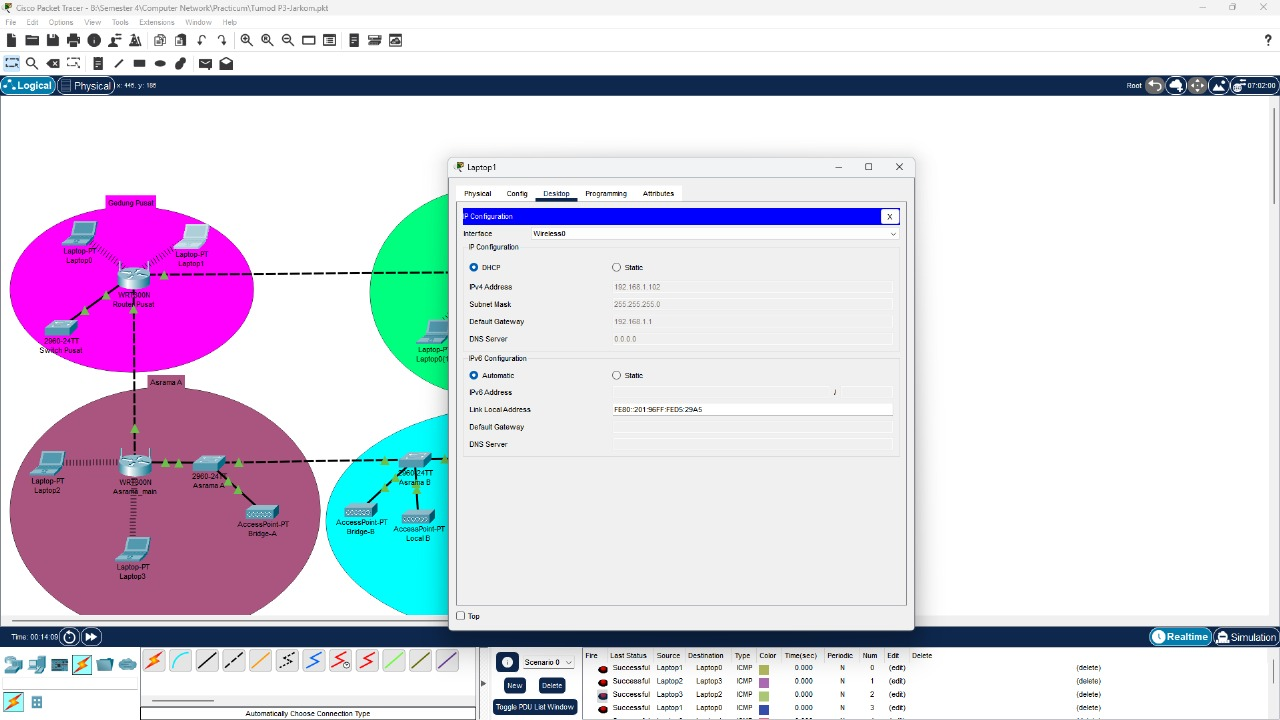
\includegraphics[width=0.6\textwidth]{img/Pusat_L.jpeg}
        \caption*{Konfigurasi Laptop Pusat}
        \label{fig:cfg_laptop_pusat}
    \end{minipage}
    \captionof{figure}{Pengaturan perangkat di Gedung Pusat. Router Pusat berfungsi sebagai gateway utama dan menyediakan konektivitas nirkabel. Laptop dikonfigurasi untuk terhubung ke jaringan ini.}
\end{figure}

\begin{figure}[h!]
    \centering
    \begin{minipage}{0.48\textwidth}
        \centering
        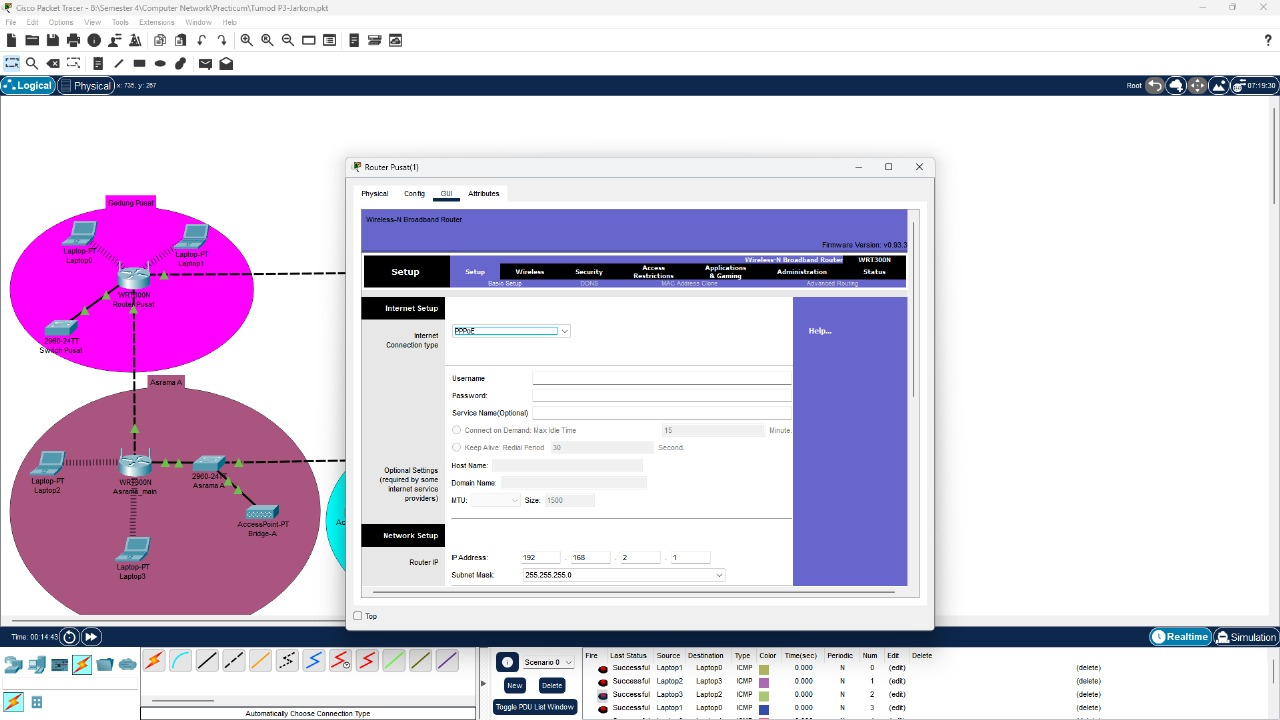
\includegraphics[width=0.6\textwidth]{img/Lab_R.jpeg}        \caption*{Konfigurasi Router Lab}
        \label{fig:cfg_router_lab}
    \end{minipage}\hfill
    \begin{minipage}{0.48\textwidth}
        \centering
        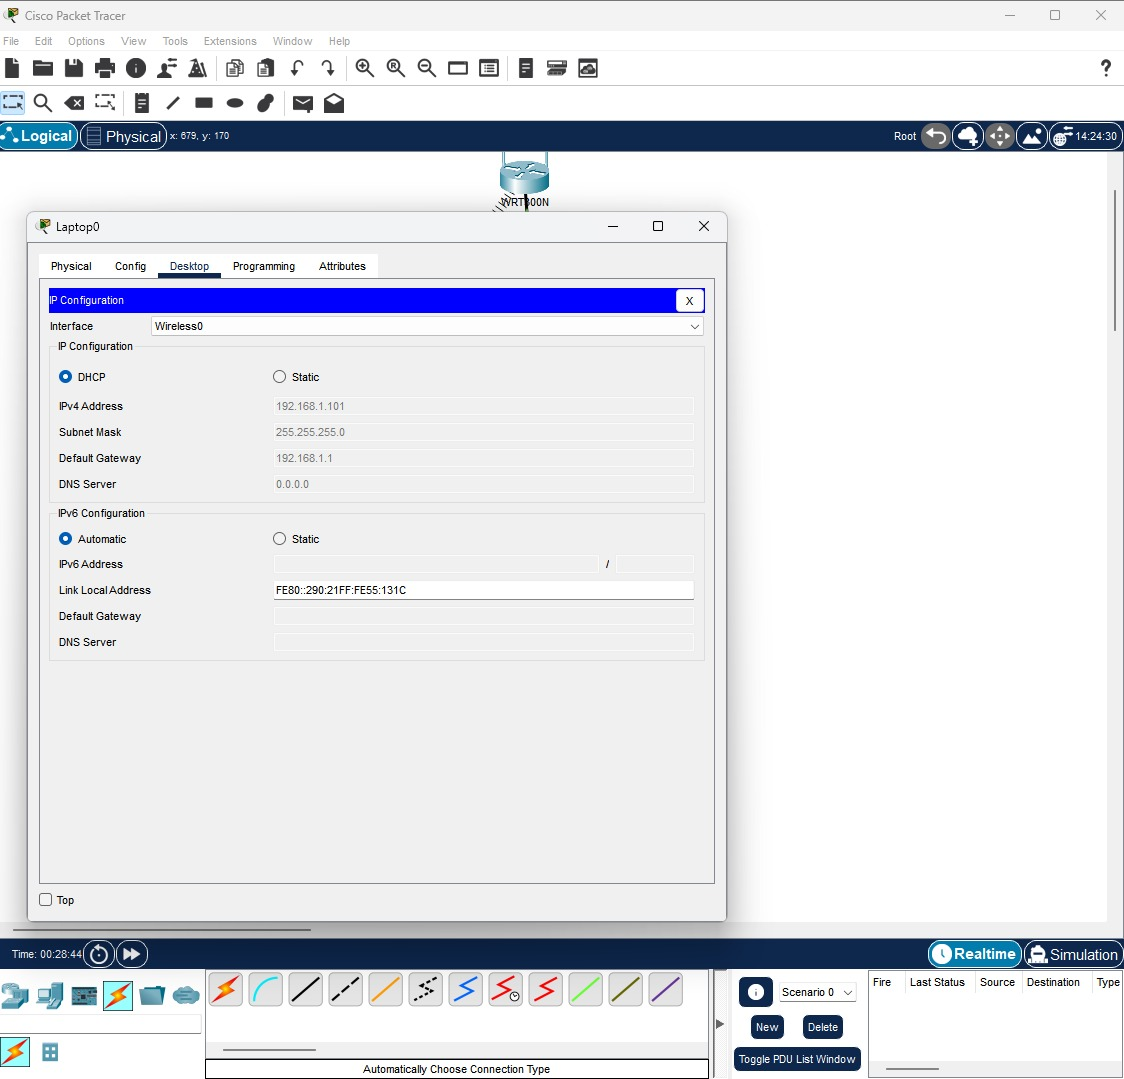
\includegraphics[width=0.6\textwidth]{img/Lab_L.jpeg}
        \caption*{Konfigurasi Laptop Lab}
        \label{fig:cfg_laptop_lab}
    \end{minipage}
    \captionof{figure}{Pengaturan perangkat di Gedung Lab. Router Lab terhubung ke jaringan Pusat melalui port WAN-nya dan menyediakan jaringan lokal untuk perangkat Lab.}
\end{figure}
\clearpage 

\begin{figure}[h!]
    \centering
    \begin{minipage}{0.48\textwidth}
        \centering
        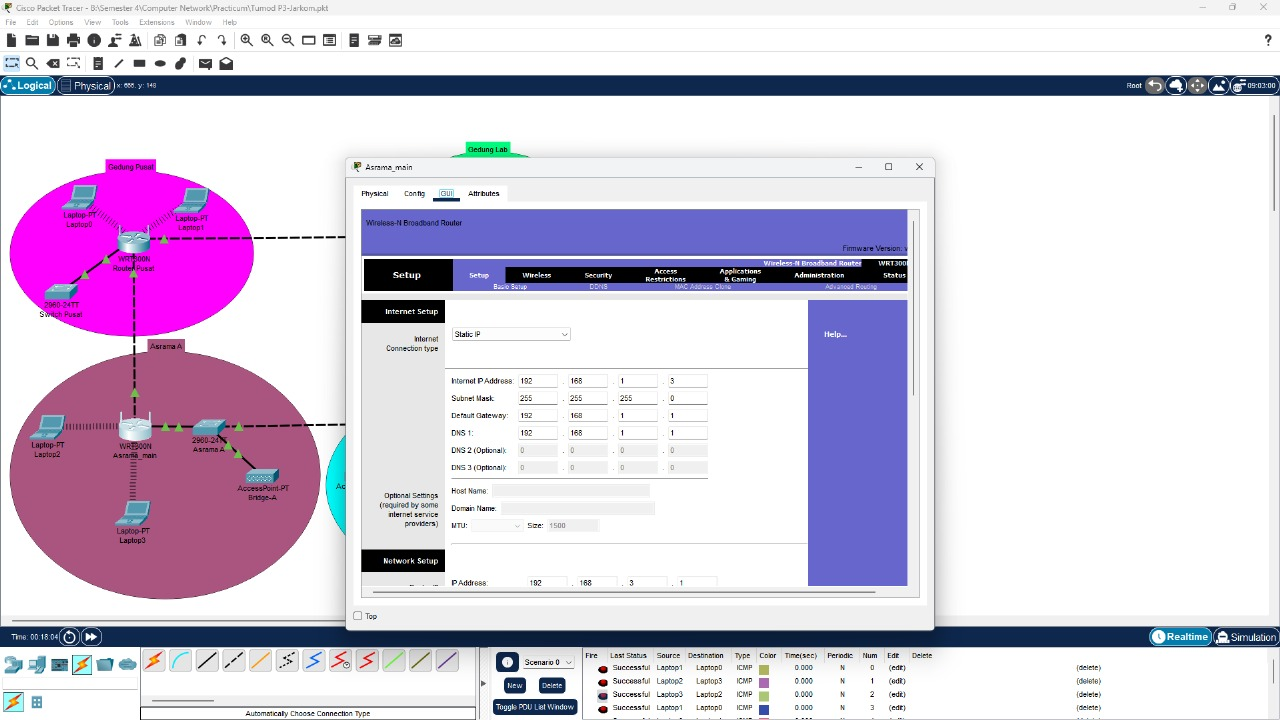
\includegraphics[width=0.48\textwidth]{img/ASA_R.jpeg}
        \caption*{Konfigurasi Router Asrama A}
        \label{fig:cfg_router_asrama_a}
    \end{minipage}\hfill
    \begin{minipage}{0.48\textwidth}
        \centering
        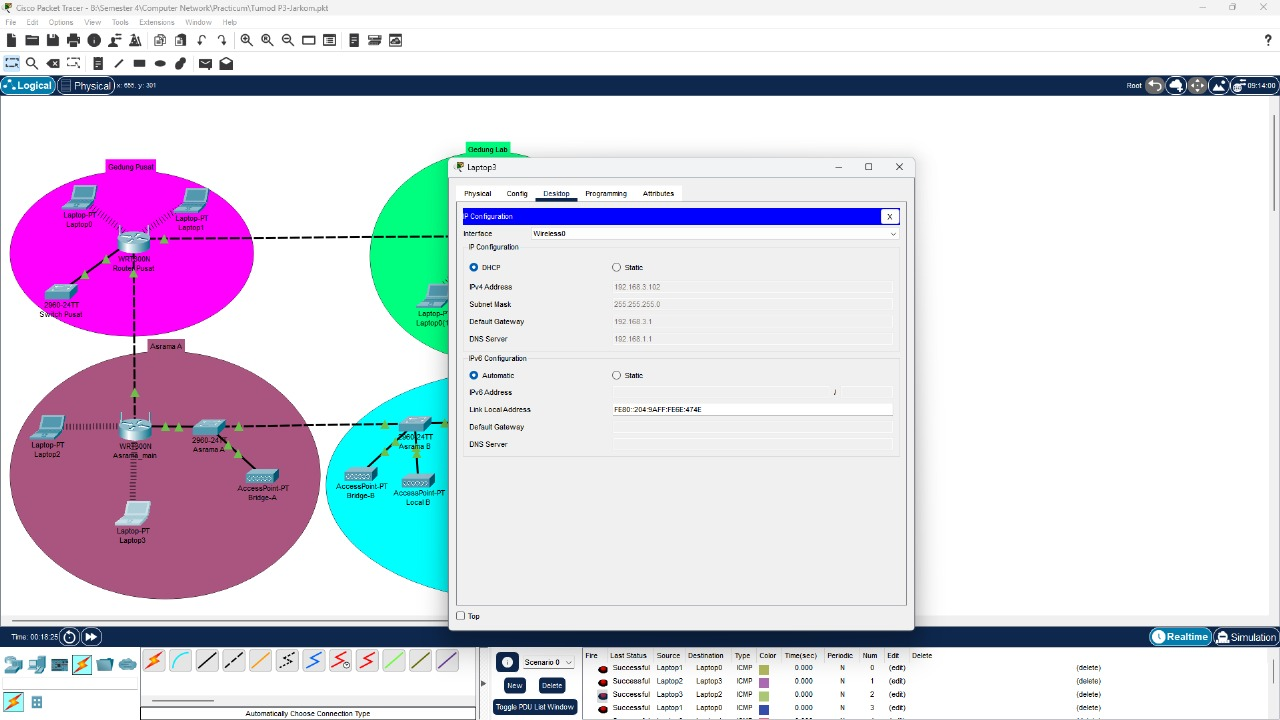
\includegraphics[width=0.48\textwidth]{img/ASA_L.jpeg}
        \caption*{Konfigurasi Laptop Asrama A}
        \label{fig:cfg_laptop_asrama_a}
    \end{minipage}
    \vspace{1em} 
    \begin{minipage}{0.48\textwidth}
        \centering
        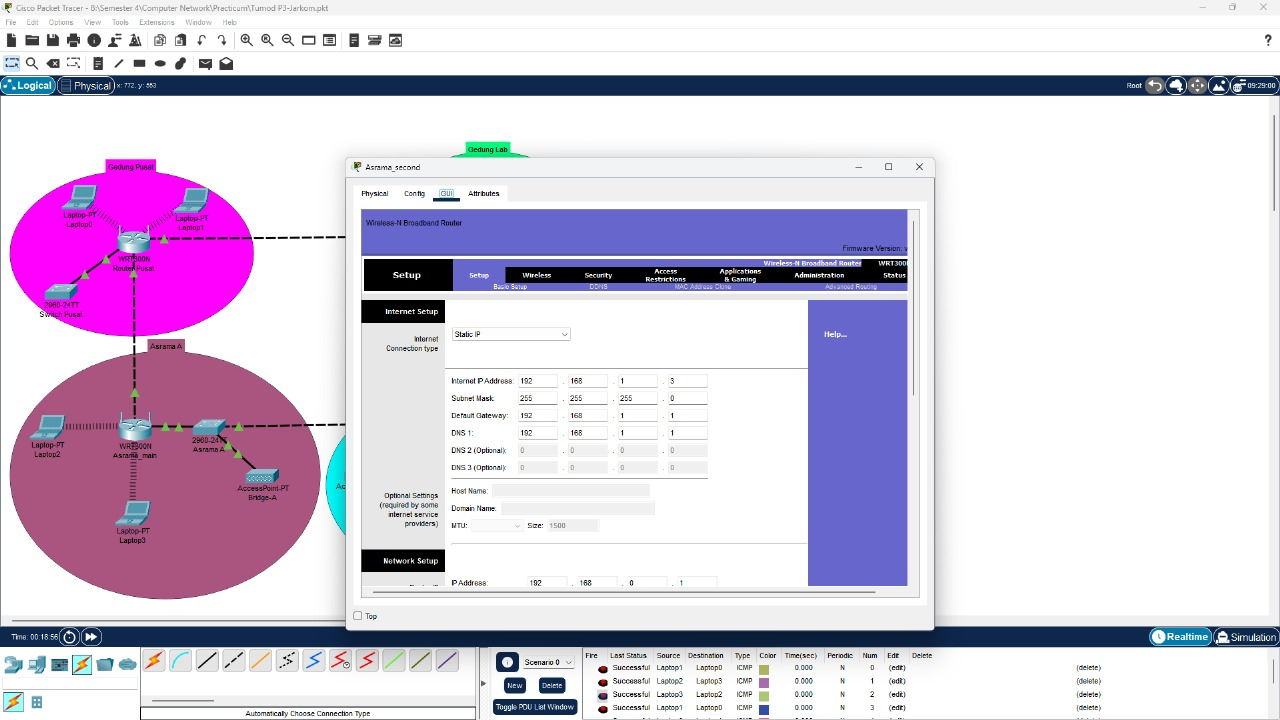
\includegraphics[width=0.48\textwidth]{img/ASB_R.jpeg}
        \caption*{Konfigurasi AP/Switch Asrama B}
        \label{fig:cfg_router_asrama_b}
    \end{minipage}\hfill
    \begin{minipage}{0.48\textwidth}
        \centering
        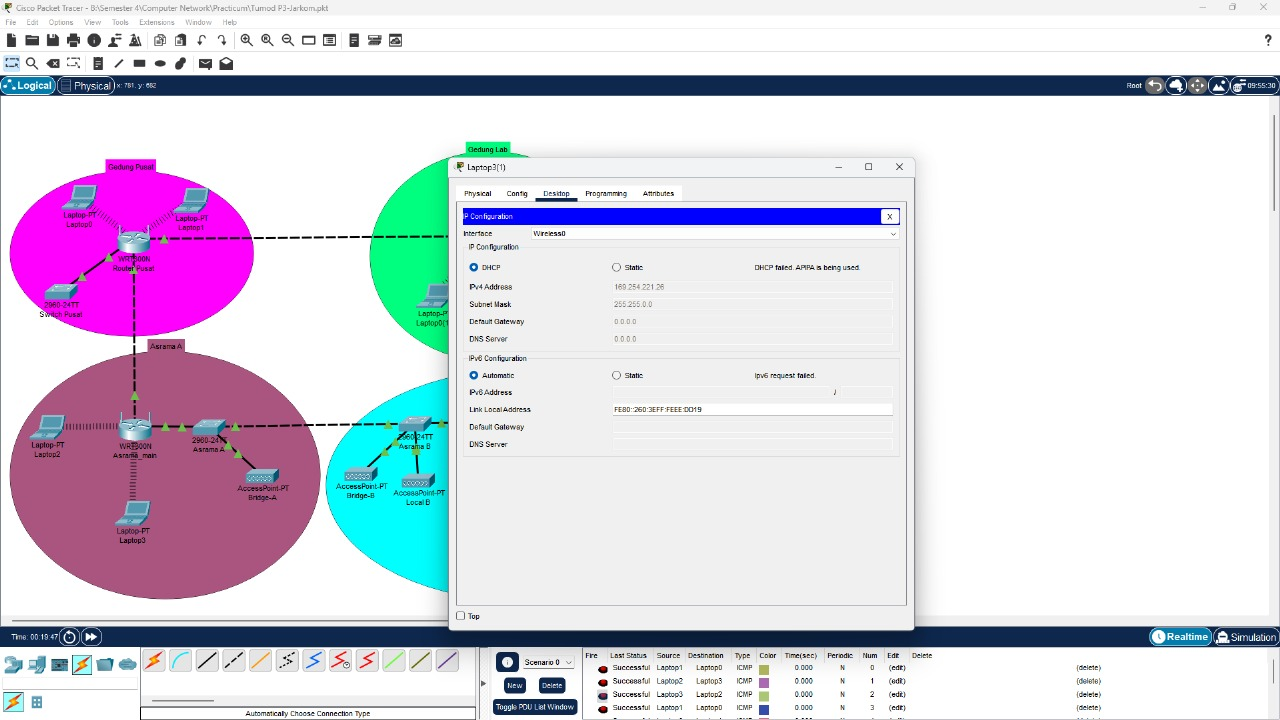
\includegraphics[width=0.48\textwidth]{img/ASB_L.jpeg}
        \caption*{Konfigurasi Laptop Asrama B}
        \label{fig:cfg_laptop_asrama_b}
    \end{minipage}
    \captionof{figure}{Pengaturan perangkat di Gedung Asrama. Router utama di Blok A mengelola jaringan Asrama secara keseluruhan dan terhubung ke Pusat. Blok B, yang terhubung ke Blok A (via kabel sebagai workaround), memiliki AP lokal untuk kliennya. Semua laptop di Asrama berada dalam satu subnet yang sama.}
\end{figure}

\subsection{Analisis dan Kendala Tugas Modul Simulasi}
Implementasi topologi jaringan antar tiga gedung ini berhasil menunjukkan konektivitas dasar antar LAN di setiap gedung dan juga konektivitas internal di dalam Gedung Asrama antara Blok A dan Blok B (menggunakan workaround kabel). Uji ping antar PC di gedung yang berbeda, yang melewati router Gedung Pusat, berhasil dilakukan setelah konfigurasi routing statis pada Router Pusat dan pengaturan WAN yang benar pada router Lab dan Asrama A.

Kendala utama yang dihadapi selama simulasi adalah:
\begin{enumerate}
    \item \textbf{Kegagalan Pembentukan Wireless Bridge Internal Asrama:} Seperti yang telah dibahas, upaya untuk menghubungkan Asrama Blok A dan Blok B menggunakan dua perangkat AP-PT sebagai wireless bridge di Cisco Packet Tracer tidak berhasil. Meskipun berbagai konfigurasi (termasuk mode open tanpa sekuriti, pencocokan SSID dan channel, serta penyesuaian jarak) telah dicoba berulang kali, link nirkabel visual maupun fungsional tidak terbentuk. Hal ini diduga disebabkan oleh keterbatasan atau bug pada simulasi perangkat AP-PT untuk skenario P2P bridge di versi Packet Tracer yang digunakan. Akhirnya, digunakan koneksi kabel Ethernet antar switch di kedua blok sebagai solusi fungsional.
    \item \textbf{Keterbatasan Fitur Router Nirkabel (WRT300N) untuk Routing Antar LAN:} Router Linksys WRT300N yang digunakan sebagai gateway di setiap gedung secara default melakukan NAT dan memiliki opsi konfigurasi routing lanjutan yang terbatas (seringkali greyed out di Packet Tracer). Hal ini menyulitkan implementasi komunikasi dua arah yang sepenuhnya terbuka antar PC di LAN yang berbeda (misalnya, PC di Lab melakukan ping ke PC di Asrama) tanpa konfigurasi tambahan seperti port forwarding (untuk layanan spesifik) atau penggantian perangkat dengan router generik yang mendukung protokol routing dinamis atau konfigurasi routing statis yang lebih fleksibel tanpa NAT. Dalam simulasi ini, fokus diberikan pada konektivitas outbound dari Lab/Asrama ke Pusat, dan konektivitas antar LAN yang dirutekan oleh Pusat.
\end{enumerate}

Meskipun terdapat kendala tersebut, simulasi ini tetap memberikan pemahaman yang baik mengenai perancangan jaringan multi-gedung, konfigurasi dasar router nirkabel, pengaturan IP addressing, dan pentingnya routing untuk menghubungkan segmen jaringan yang berbeda. Penggunaan workaround untuk bridge internal Asrama juga menunjukkan pentingnya adaptasi dalam menghadapi keterbatasan alat simulasi.

\section{Kesimpulan}
Praktikum ini menunjukkan bahwa koneksi nirkabel dapat diimplementasikan dalam berbagai mode dengan fungsi yang spesifik. Mode Point-to-Point menghubungkan dua perangkat secara langsung, Point-to-Multipoint memungkinkan satu titik akses melayani beberapa klien, dan Wireless Bridge menggabungkan dua segmen LAN. Dari praktikum ini, dapat juga disimpulkan bahwa konfigurasi awal untuk routing nirkabel cenderung lebih sederhana dibandingkan dengan implementasi jaringan berkabel, khususnya terkait aspek fisik instalasi media.

\newpage
\section{Lampiran}
\subsection*{Dokumentasi saat praktikum}
\addcontentsline{toc}{subsection}{Dokumentasi saat praktikum}
Berikut adalah dokumentasi saat praktikum Modul 3 berlangsung
\begin{figure}[h!]
    \centering
    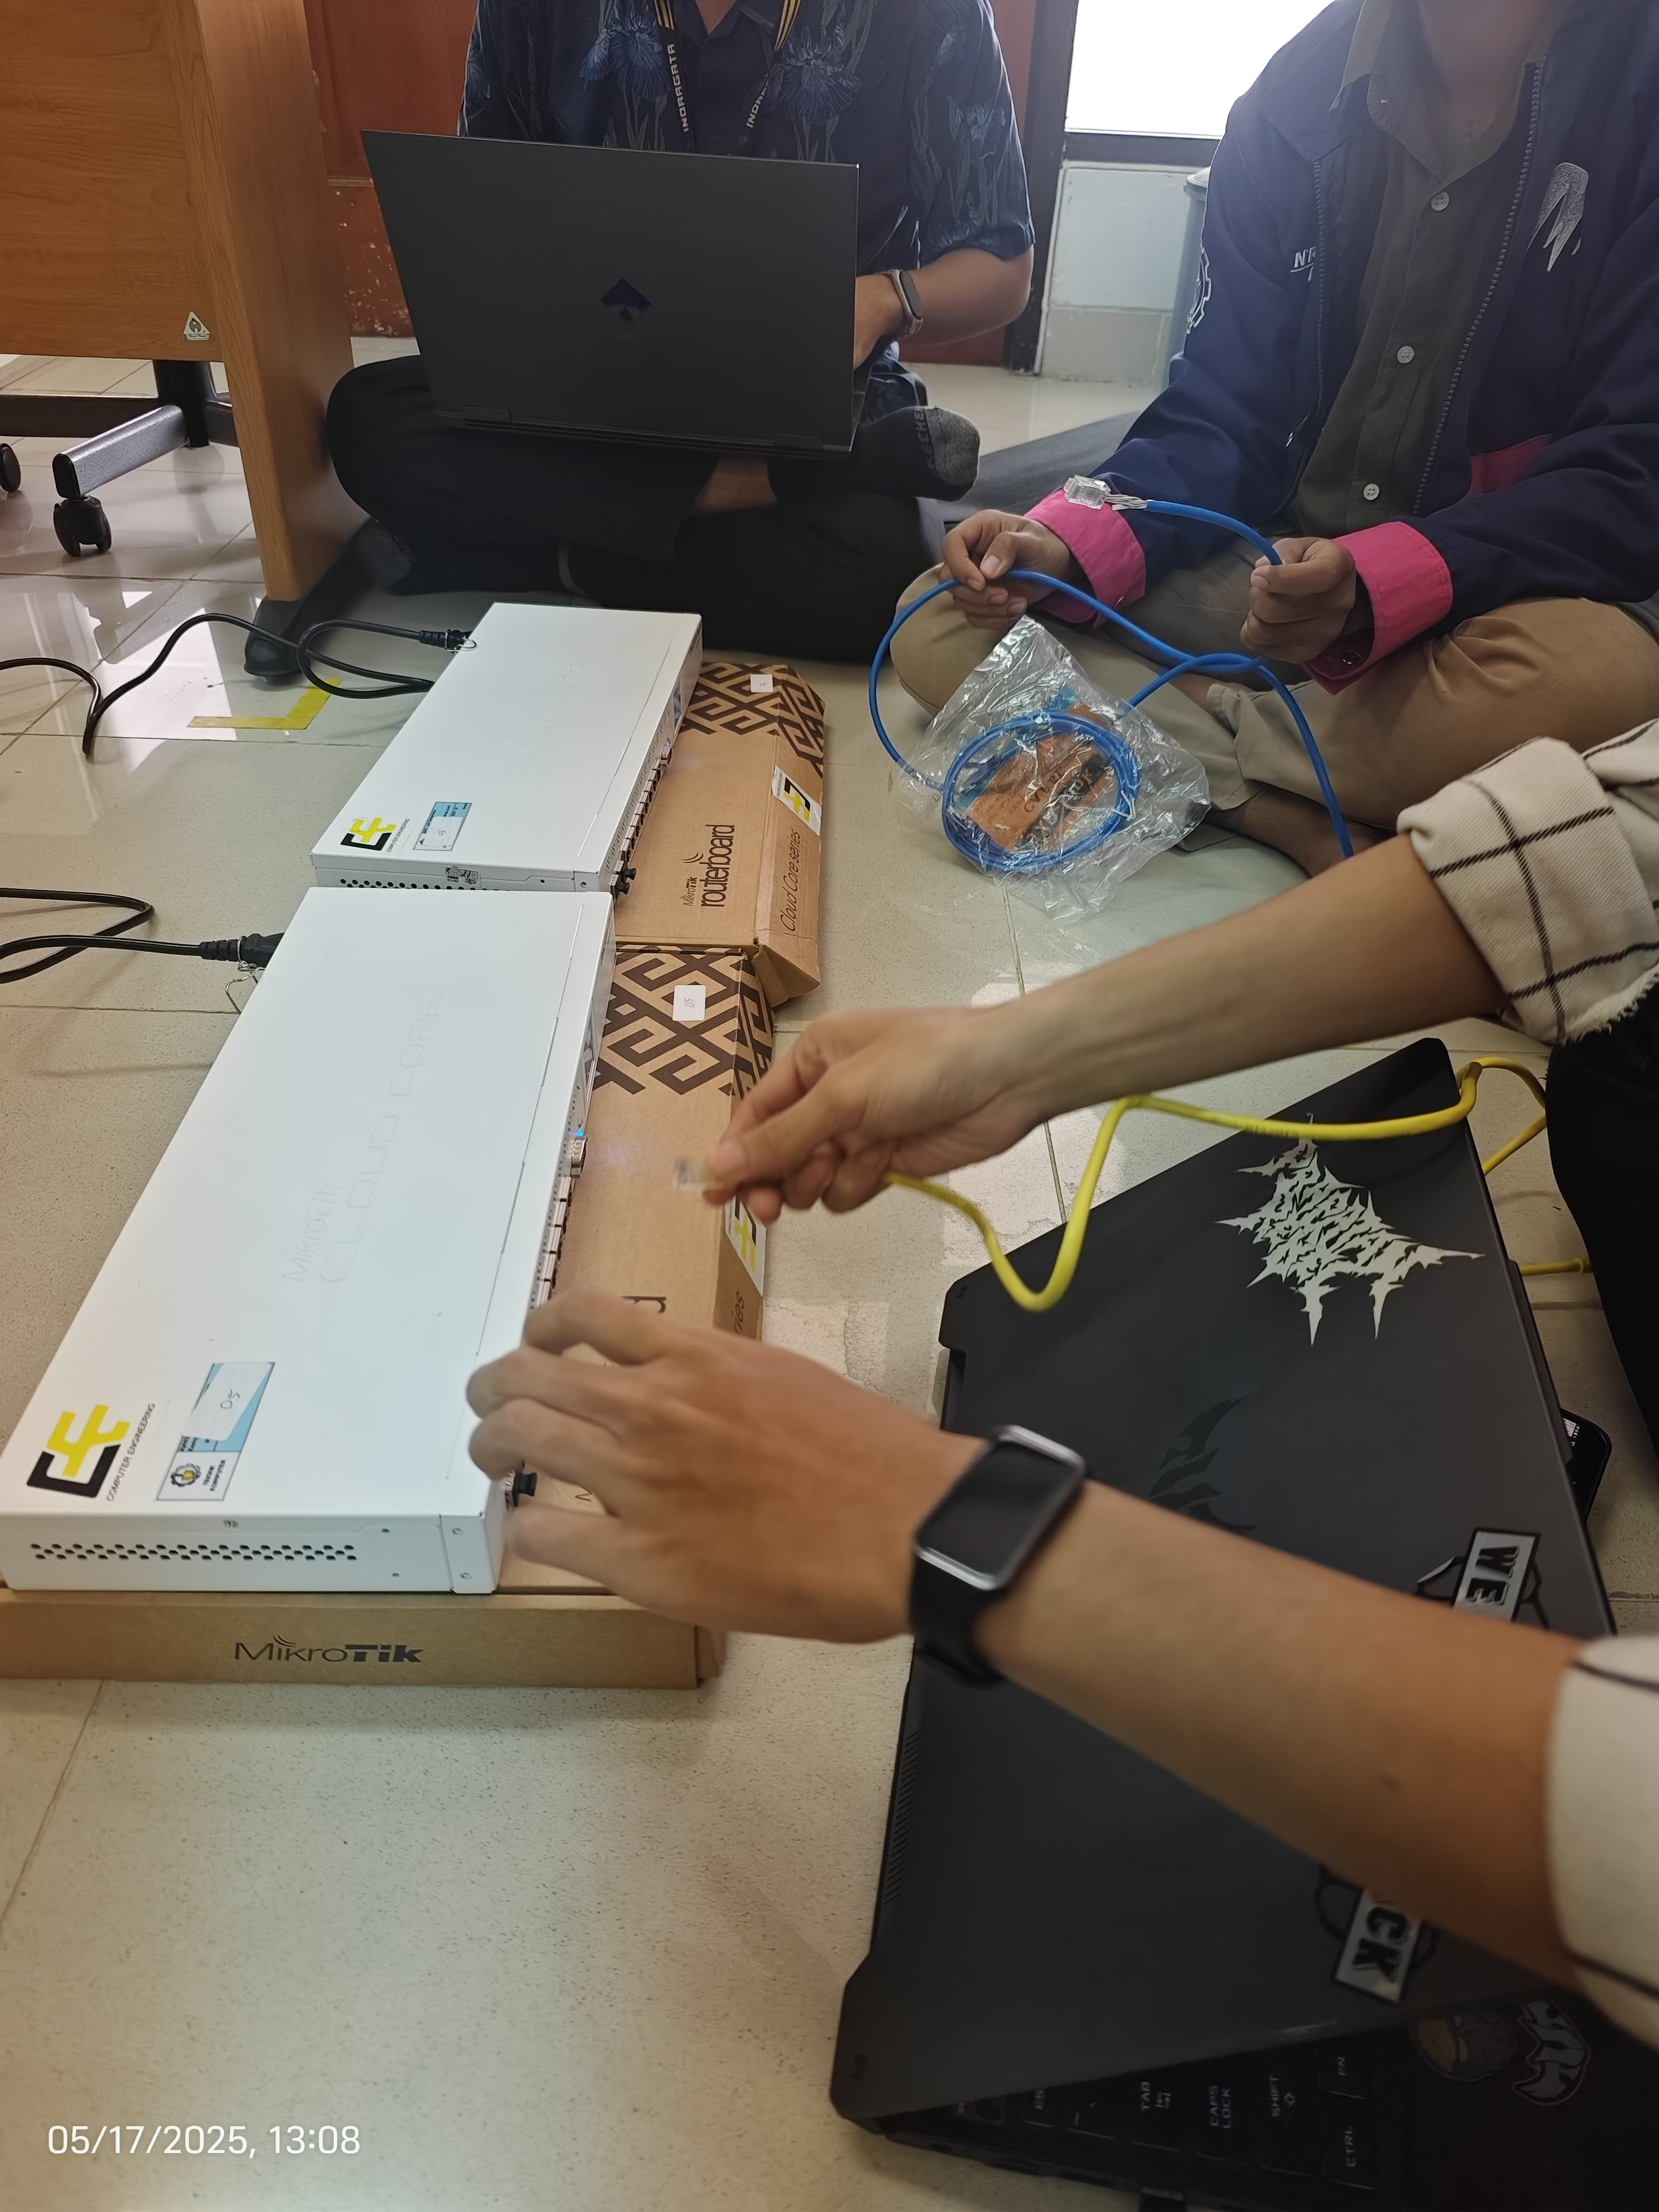
\includegraphics[width=0.7\textwidth]{img/Lampiran3.jpeg} 
    \caption{Dokumentasi.}
    \label{fig:ping_tambahan_lampiran}
\end{figure}

\end{document}


